\chapter{Linear and Logistic Regression}
%\begin{refsection}

\begin{figure}[h!]
\centering
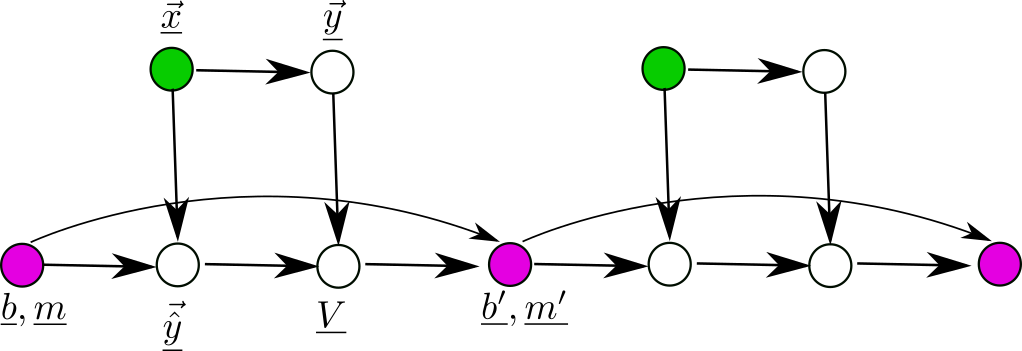
\includegraphics[width=5in]{linreg/linreg.png}
\caption{Linear Regression} 
\label{fig-linreg}
\end{figure}

\begin{figure}[h!]
\centering
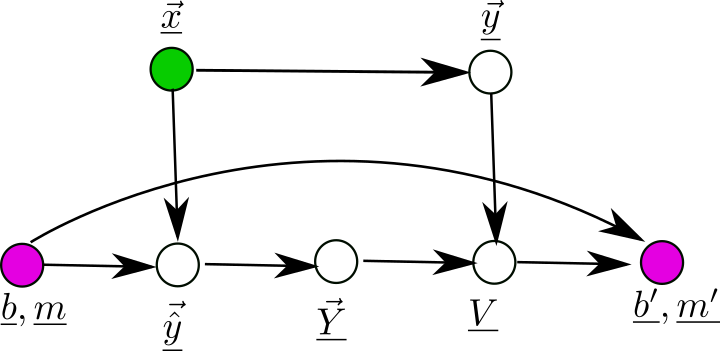
\includegraphics[width=3in]{linreg/linreg-emul.png}
\caption{B net of Fig.\ref{fig-linreg}  with new $\vec{\ul{Y}}$ node.}\label{fig-linreg-emul}
\end{figure}



Estimators $\hat{y}$ for linear and logistic regression.
\begin{itemize}
\item 

\textbf{Linear Regression:} $y\in \RR$. Note $\hat{y}\in \RR$. $(x,\hat{y}(x))$ is a straight line with y-intercept $b$ and slope $m$.
\beq
\hat{y}(x;b, m)= b + mx
\eeq

\item
\textbf{Logistic Regression:} $y\in\{0, 1\}$. Note $\hat{y}\in [0,1]$. $
(x,\hat{y}(x))$ is a sigmoid. Often in literature, $b,m$ are replaced by $\beta_0, \beta_1$. 
\beq
\hat{y}(x;b, m)=
\frac{1}{1+e^{-(b + m x)}}
\eeq
\end{itemize}

Define
\beq
V(b, m)=\sum_{x,y}P(x,y)| y-\hat{y}(x;b, m)|^2
\;.\label{eq-norm-cost}
\eeq
We want to minimize $V(b,m)$ (called a cost or loss function) wrt $b$ and $m$.


Node transition probabilities of B net of Fig.\ref{fig-linreg} given next in blue.

\beq\color{blue}
P(b,m) = \;{\rm given}
\eeq


\beq\color{blue}
P(\vecx)=\prod_i P(x[i])
\eeq

\beq\color{blue}
P(\vecy|\vecx)=\prod_i P(y[i]|x[i])
\eeq

\beq\color{blue}
P(\vec{\hat{y}}|\vecx, b, m)=\prod_i \delta(\hat{y}[i], \hat{y}(x[i],b,m))
\label{eq-replace1}
\eeq

\beq\color{blue}
P(V|\vec{\hat{y}}, \vecy)=
\delta(V, \frac{1}{nsam(\vecx)}\log \prod_i |\hat{y}[i]-y[i]|^2)
\label{eq-replace2}
\eeq
Let $\eta_b, \eta_m>0$. For $x=b,m$, if $x'-x=\Delta x = -\eta\frac{\partial V}{\partial x}$, then $\Delta V\approx \frac{-1}{\eta}(\Delta x)^2   \leq 0$ for $\eta>0$. This is called ``gradient descent".	
\beq\color{blue}
P(b'|V, b)=\delta(b', b-\eta_b\partial_b V)
\eeq
\beq\color{blue}
P(m'|V, m)=\delta(m', m-\eta_m\partial_m V)
\eeq


\begin{center}
\LARGE\textbf{{Generalization to $x$ with multiple components(features)}}
\end{center}
 Suppose that for each sample $i$, instead of $x[i]$ being a scalar, it has $n$ components called features:

 \beq
x[i] = (x_0[i], x_1[i], x_2[i] , \ldots x_{n-1}[i])
\;.\eeq

Slope $m$ is replaced by weights  

\beq
w = (w_0, w_1, w_3, , \ldots, w_{n-1})
\;,\eeq
and the product of 2  scalars $mx[i]$ is replaced by the inner vector product $w^Tx[i]$. 
\begin{center}
\LARGE\textbf{{Alternative $V(b,m)$ for logistic regression}} 
\end{center}
For logistic regression, since $y[i]\in \{0,1\}$ and $\hat{y}[i]\in [0,1]$ are both in the interval $[0,1]$, they can be interpreted as probabilities. Define 
probability distributions $p[i](x)$ and
$\hat{p}[i](x)$ for $x\in \{0,1\}$ by
\beq
p[i](1)=y[i],\;\;\; p[i](0)=1-y[i]
\eeq

\beq
\hat{p}[i](1)=\hat{y}[i],\;\;\; \hat{p}[i](0)=1-\hat{y}[i]
\eeq
Then for logistic regression, the following 2 cost functions $V(b,m)$
can be used as alternatives to the cost function Eq.(\ref{eq-norm-cost}) previously given.

\beq
V(b, m)= \frac{1}{nsam(\vecx)}\sum_i D_{KL}(p[i]\parallel \hat{p}[i])
\eeq

and

\beqa
V(b, m)&=&\frac{1}{nsam(\vecx)} \sum_i CE(p[i]\rarrow \hat{p}[i])\\
&=& \frac{-1}{nsam(\vecx)}\sum_i \left\{
y[i]\log \hat{y}[i] +
(1-y[i])\log (1- \hat{y}[i])\right\}\\
&=&
\frac{-1}{nsam(\vecx)}\sum_i 
\log \left\{\hat{y}[i]^{y[i]}(1- \hat{y}[i])^{(1-y[i])}\right\}\\
&=&
\frac{-1}{nsam(\vecx)}\sum_i 
\log P(\ul{Y}=y[i]|\hat{y}=\hat{y}[i])\\
&=&
-\sum_{x,y} P(x, y)
\log P(\ul{Y}=y|\hat{y}=\hat{y}(x,b,m))
\eeqa

Above, we used 
\beq
P(\ul{Y}=Y|\hat{y}) = \hat{y}^{Y}
[1-\hat{y}]^{1-Y}
\eeq
for $Y\in S_{\ul{Y}}=\{0,1\}$. (Bernoulli distribution).

There is no node corresponding to $\ul{Y}$
in the B net of Fig.\ref{fig-linreg}. Fig.\ref{fig-linreg-emul} shows a new B net that has a new node called $\vec{\ul{Y}}$ compared to the B net of Fig.\ref{fig-linreg}. One defines the transition probabilities for all nodes of Fig.\ref{fig-linreg-emul} except $\vec{\ul{Y}}$ and $\ul{V}$ the same as for Fig.\ref{fig-linreg}. For $\vec{\ul{Y}}$ and $\ul{V}$, one defines

\beq\color{blue}
P(Y[i]|\vec{\hat{y}})=
P(\ul{Y}=Y[i]|\hat{y}[i])
\eeq

\beq\color{blue}
P(V|\vec{Y}, \vecy)=
\delta(V, \frac{-1}{nsam(\vec{x})}\log \call)
\;,
\eeq
where $\call =\prod_i P(\ul{Y}=y[i]|\hat{y}[i] )$=likelihood.





%\printbibliography[heading=subbibliography]
%\end{refsection}